% declare documents and packages
\documentclass[man, 12pt, a4paper, nolmodern, noextraspace]{apa6}
\usepackage[T1]{fontenc} 
\usepackage[utf8]{inputenc}
\usepackage{newunicodechar}
\usepackage[american]{babel}
\usepackage{csquotes}
\usepackage{amsmath}
\usepackage{amssymb}
\usepackage{microtype}
\usepackage{caption}
\usepackage{subcaption}
\usepackage{graphicx}
\usepackage{url}
\usepackage{times}
\usepackage{booktabs}
\usepackage{multirow} % multirow tables
\usepackage{arydshln} % dashline in tabular 
\usepackage{rotating} % vertical tables
\usepackage{pdflscape} % landscape pages
\renewcommand{\footnotesize}{\small} % use 11pt for footnotes
\usepackage[doublespacing]{setspace} % single space for footnotes
\setlength{\skip\footins}{1.5pc plus 1pt} % some more space between footnote and main body
% this command put all footnotes to endnote at the end of the paper
%\usepackage{endnotes}
%\let\footnote\endnote

% for word counts
\newcommand{\detailtexcount}{%
  \immediate\write18{texcount -merge -sum -incbib -dir \jobname.tex > \jobname.wcdetail }%
  \verbatiminput{\jobname.wcdetail}%
}
\newcommand{\quickwordcount}{%
  \immediate\write18{texcount -1 -sum -merge \jobname.tex > \jobname-words.sum }%
  \input{\jobname-words.sum} words%
}
\newcommand{\quickcharcount}{%
  \immediate\write18{texcount -1 -sum -merge -char \jobname.tex > \jobname-chars.sum }%
  \input{\jobname-chars.sum} characters (not including spaces)%
}

% Biblatex
\usepackage[style=apa,sortcites=true,sorting=nyt,backend=biber,uniquename=false]{biblatex}
\AtEveryBibitem{%
  \clearfield{issn} % Remove issn
  \clearfield{doi} % Remove doi
  }
% make in-text citations clickable
\usepackage[colorlinks=true]{hyperref}
% this removes annoying colors for in-text citation entries 
\usepackage{xcolor}
\hypersetup{  
    colorlinks,
    linkcolor={red!50!black},
    citecolor={blue!50!black},
    urlcolor={blue!80!black}
}

\addbibresource{CCR_lit.bib}
\DeclareLanguageMapping{american}{american-apa}
 
\title{When Does Garbage Start to Stink? Imperfect Gold Standards and the Validation of Automated Content Analysis}

\shorttitle{When Does Garbage Stink?}


\author{\addvspace{.25in} Hyunjin Song, Petro Tolochko, Jakob-Moritz Eberl, Olga Eisele, Esther Greussing, \\
        Tobias Heidenreich, Fabienne Lind, Sebastian Galyga, and Hajo G. Boomgaarden}

\affiliation{Department of Communication, University of Vienna, Austria}

\abstract{
Automated text analysis methods become increasingly popular for analyzing texts in the social sciences. However, with the growing popularity of such approaches, the issue of the validity of obtained results and the conclusions drawn from them becomes crucial: Blindly applying automated approaches, and hence feeding algorithms into the machine without proper validation, may result in misleading or even plainly wrong findings. Against this backdrop, this study first presents a systematic review of articles published in the major social science journals in the past 20 years, showing that the current practices of validation are far from being acknowledged in the literature and that the reporting and interpretation of validation procedures differ greatly. In a second step, we assess the previously unexplored connection between the quality of human judgment and relative performance of automated procedures (against true standards) by relying on large-scale, systematic Monte-Carlo simulations. Results confirm the expectation that any decision taken in terms of data preparation weight toward the quality of results one is able to obtain from automated text analysis. Our contribution should therefore be read as a call for a systematic application of validation procedures in any social science publication drawing on automated text analysis procedures.
}

\keywords{Automated text analysis, reliability, validation, Monte-Carlo simulations}

\authornote{Please direct any questions and inquiries concerning this manuscript to \href{mailto:hyunjin.song@univie.ac.at}{hyunjin.song@univie.ac.at}}

\note{\addvspace{.25in} 
Draft date: \today \\
\addvspace{1in} 
Paper prepared for Inaugural issue of Computational Communication Research  \\
\addvspace{.25in} 
      \textbf{Draft in progress. Please do not cite without permission.} \\
      }

\begin{document}
    
\setcounter{page}{0}
\maketitle

    Automated text analysis methods become increasingly popular for analyzing texts in the social sciences, ranging from large-scale analyses of decades of newspaper coverage and party manifestos to millions of social media posts. Taking advantage of the fact that ever-growing quantities of text are available yet available resources are usually limited, research in the social sciences nowadays readily turns to automated approaches to investigate a great range of questions in manifold sources \parencite{Boumans_Trilling_2016, grimmer2013text}. However, with the growing popularity of such approaches, the issue of the validity of obtained results and the conclusions drawn from them becomes crucial. Blindly applying automated approaches, and hence feeding algorithms or dictionaries into the machine without proper validation, may result in misleading or even plainly wrong findings; a principle famously illustrated by the phrase \enquote{garbage in, garbage out.}
    
    In this regard, such \enquote{text-as-data} approaches squarely depend on a proper validation of applied techniques against some gold-standard \parencite{grimmer2013text}.\footnote{Here, we use the term \enquote{gold-standard} and \enquote{ground truth} largely interchangeably, denoting some forms of objective data that serve as the reference.} Typically, applications of validation procedures using gold-standards rely on some human inputs (\enquote{human coding}) as a  benchmark to systematically compare and evaluate against proposed supervised methods-based or dictionary-based classifications. Acting under the assumption that humans’ understanding of text outperforms that of machines and that, if trained correctly, humans will make mostly correct and valid classifications of texts, human coded data is treated as a gold-standard against which the performance of the computer is judged. However, “the quantities we seek to estimate from text [\ldots] are fundamentally unobservable” \parencite[p. 299]{lowe2013validating}, and human judgment is, in fact, no exception to this general rule --- as we know from the methodological content analysis literature. The consequences of, for example, human biases, predispositions and situational disturbances resulting in differing levels of “reliability” in human judgment in evaluating texts are well documented in traditional content-analytic applications \parencite[e.g.,][]{krippendorff2004reliability, hayes2007answering, lombard2002content, ennser2018impact}. Hence, the gold-standard might not be as shiny as oftentimes assumed. By conditioning the relative performances of a given automated method against human inputs, we argue, the imperfect human coding (imperfect “gold-standard”) greatly percolates a potentially already imperfect estimation of the automated procedures. Yet, the implications of using such imperfect human judgments as the benchmark for evaluating the validity of the results of automated text analysis – and especially the consequences of different levels of reliability in the gold-standard manually materials are, until today, still insufficiently addressed.
    
    Against this backdrop, we first presents a systematic review of articles published in the major social science journals in the past 20 years, showing that the actual practices of systematic validation are far from being acknowledged as a standard in the literature, and that the reporting and interpretation of validation procedures differ greatly. More importantly, in a second step, we argue that using imperfect human judgments as the benchmark effectively \enquote{tolerates} any mistakes or classification errors of automated procedures to a degree comparable to imperfect human judgments, which may have systematic consequences for the evaluation of the proposed automatic procedures. We assess this previously unexplored connection between the quality of human judgment and relative performance of automated procedures (against true standards) by relying on large-scale, systematic Monte-Carlo simulations. To our knowledge, our contribution is among the very first to provide a thorough, systematic evidence pertaining to a well-known, yet extremely scarcely discussed topic in automated content analysis. Our contribution should be read as a call for a systematic application of validation procedures in any social science publication drawing on automated text analysis procedures. At the same time, the study serves to benchmark the combination of reliability in gold-standard/ground truth and validity scores and warns against improper use of both to demonstrate the validity of the approach. 
    
\section{Logics and Procedures of Automated Content Analysis}

    We define \enquote{automated content analysis} (or automated text analysis) as the collection of content-analytic approaches that utilize automated methods of coding a large amount of unstructured textual data, in a way that the coding process itself (i.e., the text classification) is not performed manually but rather done by predefined computational algorithms \parencite{trilling2018scaling, grimmer2013text}. While the usage of the term \enquote{automated content analysis} in general in the extant literature encompasses a wide variety of forms \parencites[e.g.,][]{riff2014analyzing, Hopkins_King2010, Krippendorff2013, grimmer2013text}, here we mainly refer to supervised machine learning methods and a simple dictionary approach. We choose to do so based on the consideration that many of the automatic content analysis applications in the social sciences in general and in communication science in particular still heavily rely on those two broad approaches, where such methods are \enquote{designed to automate the hand coding of documents\ldots[in a way that] it will directly replicate the hand coding} \parencites[][p. 13]{grimmer2013text}. At the presence of a large volume of data, this can be an attractive option for overcoming the inherent time and resources constraints in manual approaches.\footnote{Whereas  dictionary-based or supervised learning methods assume already well-defined categories, the unsupervised methods such as LDA topic modeling \parencites[][]{dimaggio2013exploiting, maier2018applying} generally aim to inductively \enquote{discover} new classifications without any human input. Since our primary interest is the interplay of human input and machine output, we do not consider such methods here. Also, our definition (inevitably) exclude automatic approaches of \textit{acquiring} data, or traditional manual content analysis but merely make use of automated procedures in tasks other than the actual coding process \parencites[such as in data entry or data management: e.g.,][]{lewis2013content}.} In addition, in practice, such methods are relatively easy to implement in combination with manual approaches, which are still the dominant workhorse for many communication scholars.
    
    Although a specific method and application of automatic content analysis comes in many flavors \parencites[for a broad overview, see:][]{Boumans_Trilling_2016, grimmer2013text}, they are all based on similar principles: they all aim to identify and classify the predefined categories (i.e., a discovery and measurement). A simple dictionary approach generally relies on the pre-defined “dictionary” of words or phrases by a researcher -- ranging from simple keywords lists to complex Boolean expression, syntactic parsers, or even regular expressions -- where the computer counts the number of such instances in a given document. Assuming a given dictionary is appropriate to be applied in a given domain \parencite{Boumans_Trilling_2016, gonzalez2015signals}, a researcher applies the dictionary on a set of documents, typically to a word-level, and then resulting \enquote{scores} are aggregated into the document level (e.g., a news article or tweet). This \enquote{dictionary} therefore represents a explicit coding rule to be applied by an algorithm, where (classified) categories may represent the visibility of a topic (i.e., the presence or the absence of a category) or a net tonality (positive vs. negative) of an article \parencites[e.g.,][]{Aaldering2016, YoungSoroka2012, boomgaaden2009, gonzalez2015signals, Rooduijn2011}. 
    
    For supervised methods, specific coding rules in manual annotations (as an input to an algorithm) are, in general, rarely explicitly articulated. Yet the algorithm takes such implicit judgments derived from manual coding as the point of reference, and tries to infer the features of data that best classify the text into different predefined categories. Currently, there exists a variety of supervised learning algorithms available -- ranging from a simple regression framework or Naïve Bayes to more sophisticated methods such as Support Vector Machines (SVM) or random decision forest \parencites[for an overview, see][]{hindman2015building}. This machine-learning process may involve many iterations of \enquote{training} and comparisons to some gold-standard materials in order to achieve a desired level of a classification quality \parencites[e.g.,][]{scharkow2013thematic}. If the algorithmic coding is later determined to be sufficient enough in capturing the underlying quantities of interest through such a \enquote{training,} then a researcher applies such \enquote{trained} coding rules to a larger corpus of unseen documents to perform their analyses \parencites[e.g.,][]{burscher2015using, burscher2014teaching, scharkow2013thematic, gonzalez2015signals}.    
    
\section{The Use of Human Coding in Cross-Validation of Automated Content Analysis}
    
    Just as the term \enquote{automated content analysis} itself, the notion of \enquote{validation} often signifies many different practices, although most of them usually involve some notions of triangulation \parencites{Neunhoeffer2018}. Yet for automated content analysis methods in particular, the discussion of \enquote{validation} has traditionally evolved around the general logic of establishing a correlative or a convergent validity of a measurement \parencites[][]{Krippendorff2008validity}. This is because any automated content analysis application -- at least the ones we are focusing on in this contribution -- essentially can be regarded as a classification problem (i.e., a measurement of the predefined categories in data). In this respect, the most straightforward method of validating a given measurement is to compare with another measurement of the same concept. Therefore, applications of validation procedures in automated content analysis have traditionally relied on some sort of human inputs (“human coding”) as a benchmark as discussed above. 
    
    In dictionary-based approaches, the actual coding process itself using the existing dictionary does not involve any human inputs.\footnote{However, a great deal of labor-intensive human inputs is required when building and constructing a well-defined dictionary \parencite{YoungSoroka2012, muddiman2018re}. Due to its labor-intensive nature, recent applications in this topic increasingly turn to \enquote{crowdcoding}, where the manual labor of highly trained yet few number of human coders are replaced with a large number of (untrained) crowd-coding workers \parencites[][]{haselmayer2017sentiment, lind2017content}.}  Instead, the use of manual coding in dictionary approaches may involve additional comparisons of the derived results against manual coding, often made \textit{post-hoc} for validating the results. A recent work by \textcite{Rooduijn2011} on the (automatic) measurement of \enquote{populism} in election manifestos well exemplifies the use of human coded data in validating the results of automated approaches. Using a traditional manual content analysis, they show that dictionary-based automatic coding of \enquote{populism} categories in party manifestos produces essentially very similar results compared to manual coding. Similarly, \textcite{YoungSoroka2012} compare the manually coded newspaper content against the results based on Lexicoder Sentiment Dictionary (LSD), and found that results using LSD and manual content analysis are largely comparable to each other.
    
    Nevertheless, it is exceptionally rare to see a validation of results \textit{after} such classification tasks \parencites[yet for notable exceptions, see][]{muddiman2018re, YoungSoroka2012, gonzalez2015signals}. Once the dictionary is created, one typically assumes the classification membership that has to be estimated by an algorithm to be a simple additive --- and exclusive --- function of the given dictionary elements (i.e., an aggregation of positive and negative dictionary scores results in the general sentiment of the article, etc.), typically ignoring any residual textual features that are not captured by a given dictionary. Such blind trust in the dictionary grossly misses the very likely possibility that a given text in question (i.e., a newspaper article or a social network post) is more than a simple sum of its parts. However, to our knowledge, little to no validation has been done in substantive studies.
    
    In supervised methods, the role of human input is more central in fine-tuning the algorithm (i.e., an \enquote{inner} cross-validation). As exemplified in \textcite{scharkow2013thematic}, in supervised methods a researcher typically produces manually annotated sample materials, or a \enquote{training set,} and the algorithmic classifier is later trained on sample material in order to develop certain statistical models (that effectively aim to reproduce implicit coding rules of human coders) to predict and classify unseen materials, the \enquote{test set.} As such, human inputs are more directly utilized in such \enquote{learning} procedures in supervised methods, as opposed to being utilized post-hoc as in dictionary approaches. For instance, \textcite{burscher2014teaching} have developed a supervised machine-learning algorithm to automatically classify certain generic media frames in news articles, based on a random subset of data that were manually coded by trained coders.\footnote{In unsupervised methods, the use of human-coding as a benchmark is a common practice as well. For instance, \textcite{lowe2013validating} directly compare direct human-coding based party position scaling (which serves as a benchmark) against unsupervised scaling methods; they found that the proposed parametric scaling methods can produce largely similar results on par with human judgments.} Yet due to inherent resource constraints associated with human coding, such validations typically rely on only a small subset of held-out samples to provide annotations that establish the ground-truth. As such, although in principle a researcher can further validate their final outcomes by relying on an additional post-hoc validation method as described in dictionary-based approaches (i.e., an \enquote{outer} validation), this is rarely offered in practice.   
    
\section{The Myth of Perfect Standard in Human Coding?}

    Regardless of its specific orientations briefly reviewed above, the use of human coding as a gold-standard is often regarded as \textit{the} principal method of ensuring the validity and soundness of conclusions derived from the proposed automated procedures \parencites[e.g., ][]{grimmer2013text, dimaggio2015adapting}. The purpose of such cross-validation against a gold-standard is, as \textcite{Krippendorff2008validity} notes, \enquote{to confer validity on the otherwise uncertain research results} (p. 6). Admittedly, this logic requires that the chosen benchmark (i.e., manual annotations by human coders) to be of \enquote{objective} and \enquote{unquestionable} truth --- which, anecdotally, is more common among natural language processing and sentiment analysis literature \parencites[][]{dimaggio2015adapting}. Yet, as much of the traditional manual content-analytic literature suggests \parencites[e.g.,][]{krippendorff2004reliability, hayes2007answering, lombard2002content, ennser2018impact}, manual coding more often easily produces unreliable judgments as well, and especially so when the judgment in hand requires a nontrivial degree of inferences and subjectivity to classify a latent information \parencites[][]{riff2014analyzing, Krippendorff2013}.       
    
    The issue of (inter-coder) reliability is one of the most essential concerns in the extant literature concerning the quality of manual content analysis. At least for many recent manual content analysis applications, there has been relatively little disagreement regarding the consequences of sub-optimal reliability for key measurements \parencites[][]{krippendorff2004reliability, Krippendorff2013}, and the need for better reliability for that matter. Yet to date, little attention has been devoted to the question of how the \enquote{quality} of manual coding affects the validity and conclusions derived from automated procedures. This is especially surprising, since \enquote{whenever ... principles by which humans generate ratings are heterogeneous across raters} \parencites[][p. 4]{dimaggio2015adapting}, any automated procedures that are systematically evaluated upon such imperfect human input will be biased to the degree that can be found in such biased human judgments. 
    
    The use of (potentially) imperfect human coding as an ultimate benchmark against automatic techniques may therefore have at least two systematic consequences. First, while automated methods themselves are perfectly reliable, imperfect human judgments (on validation materials) essentially makes the ultimate \enquote{target} of such perfectly reliable measurements radically deviate from the \enquote{true} target of inference, making them \enquote{reliably wrong} on-target. Second, and somewhat relatedly, systematically flawed human judgment can bias the performance of learning algorithms, leading to biased conclusions against a true standard. Therefore, using imperfect human coded data as an ultimate benchmark makes it harder to evaluate the relative trustworthiness of such validation procedures. However, most of the studies do not provide any validation at all (please see our later empirical section), or even among studies which \textit{do} compare automated procedures with manual coding as a validation tool, they often misreport or misspecify the validation metrics and hardly ever report the quality of such manual coding itself but essentially treat such imperfect human judgment as \textit{the} unquestionable truth \parencites[e.g.,][]{gonzalez2015signals, lowe2013validating, YoungSoroka2012}. Indeed, we know only one existing study that suggests some tentative evidence between quality of human coding and (machine-based) classification accuracy \parencite{burscher2014teaching}.\footnote{In a recent study, \textcite{gonzalez2015signals} compare five available sentiment dictionaries against human annotations, yet they do not directly deal with the implications of imperfect reliability in human coding. \textcite{scharkow2017measurement}, the only one of existing studies that examines the consequences of imperfect reliability in human coding, mainly deal with its implication on \enquote{linkage analysis}, but not on automated content analysis.}     
   
    In sum, there appears to be a convincing reason to suspect a systematic relationship between the quality of human coding and the relative bias and errors regarding the ultimate conclusions from the automated content analysis -- especially when using such imperfect human coding as the ``gold-standard''. While many of prior contributions on this topic -- both theoretically and empirically -- stresses a need for a proper validation of applied techniques against some gold-standard \parencites[e.g.,][]{grimmer2013text, Hopkins_King2010, gonzalez2015signals}, we do not know much about how the field in general stands in terms of standard validation practices and the use of imperfect human coding in particular. Therefore, we first conduct a systematic review of relevant articles published in the top social science journals in the past 20 years, focusing on the use of manual coding (by trained human coders), if any, in standard validation procedures against the proposed automated methods, and the assessment of performances of such automated methods (Study 1). While this systematic review should provide us an overall picture of typical validation procedures in any publication drawing on automated text analysis procedures in extant literature, study 1 at the same time further serves to benchmark in modeling the combination of reliability in manual coding and validity scores against the true standard (Study 2), where we warn against improper use of both to demonstrate the validity of the approach.

\section{Study 1: A Content Analysis Study}

\subsection{Sample and Procedures}

    We have identified relevant studies using the EBSCO host databases “Communication \& Mass Media Complete,” “Humanities Source,” and “SocINDEX with Full Index,” querying all abstracts and keywords using the following Boolean search string: \textit{("computer assisted" OR "automated" OR "automatic" OR "computational" OR "machine learning") AND ("content analysis" OR "text analysis")}. This resulted in a total of 192 identified English-language journal articles between January 1, 1998 and November 7, 2018. Among them, 119 articles were determined not relevant (e.g., an overview/introduction article, qualitative analysis, or studies using unsupervised methods or simple keyword frequencies, etc) and 7 articles were either duplicates or did not contain full texts. These articles were therefore excluded from further analyses. Using remaining 73 articles, we systemically examined whether extant applied studies using dictionary- or supervised methods a) adequately employ any cross-validation of their primary findings, b) if so, whether they use human coded materials as a benchmark, and c) if so, whether intercoder reliability and other methodological details are adequately and consistently reported. 
    
    A total of five highly qualified coders tested the initial coding scheme by independently coding 10 sample articles (approximately 14\% of total sample) and collectively discussed any coding problems and disagreement. Based on this iterative procedure, coding instructions were revised until the coding schemes would produce reliable results among any trained and competent coders. Intercoder reliability was assessed and reached Krippendorff’s alpha level of above 0.75 for each of the variables coded.   
    
\subsection{Results}

    The results of the systematic literature review are presented in Table \ref{tab:Table1} below. Specifically, 55 of the studies identified as relevant used methods related to dictionary approaches, while 18 used supervised machine learning. Only about half of the papers using a dictionary approach to automated content analysis referred to some sort of manual gold standard in their text, and even less – only 16 per cent – actually reported measures of inter-coder reliability. Notably, shares are much higher when coming to papers using supervised machine learning. The most common measure of inter-coder reliability reported were percentage agreement (in seven cases), with an average value of 0.87, and Krippendorff’s alpha (in six cases), with an average value of 0.64.
    
    When it comes to the papers referring to procedures of validation of their automated approaches, results were very similar. However, only around 40 percent of papers using a dictionary approach also reported the validation measures, compared to 67 percent of papers using supervised machine learning. Although the most commonly used measures of validity are the widely accepted measures of precision (in 13 cases, M = 0.74) and recall (in 9 cases, M = 0.60), other metrics were used as well. This is disconcerting insofar as these other measures tend to be used for testing the reliability of manual coding (e.g., Holsti, Cohen’s Kappa, Krippendorff’s alpha). Some papers only report correlation coefficients. Very generally, the result reveals that reported measures of validation do not always meet the requirements when it comes to properly assessing the quality of \enquote{gold-standard} materials and assessing the validity of automated coding.
    \centerline{ -- Table \ref{tab:Table1} about here -- }    

\section{Study 2: A Monte-Carlo Simulation Study}
    
    The result of Study 1 reveals \textcolor{red}{TBA}. 
    
    In order to systematically evaluate how different setups and practices of utilizing manual coding within automated procedures can yield different conclusions, we setup an extensive set of Monte Carlo (MC) simulations (\textit{N} = 240,000). MC simulation offers a convenient tool for systematically evaluating the relative bias and coverage of a given statistic under certain scenarios \parencites[for an example, see][]{scharkow2017measurement, leemann2017extending}. 
    
    While we based our procedures in a way that largely mirrors the typical approaches in this area, dictionary approaches and supervised learning approaches considerably differ in how they utilize manual coding, as well as their data requirements and the logic underlying each of the technique. Therefore, here we have developed two separate approaches in simulating their behaviors. Yet in all of the cases, we have broken down our approach into three stages – data generation, human coding, and automatic classification – where we systematically varied the intercoder reliability of the “gold-standard” material, along with a number of related factors such as the number of coders and the number of manual annotations per coder (see below section). Then we systematically compared different scenarios in terms of their classification accuracy and F1 scores (i.e., precision and recall) based on the \enquote{true} standard (i.e., a quantity of interest that is typically unknown to researchers) in order to illustrate how different practices of human coding in automated content analyses affect the overall results and the relative trustworthiness of conclusion drawn from such results.
    
    \subsection{Data Generation Stage}
    
    We create data (e.g., textual data to be analyzed by a researcher) with the \enquote{true} outcome variable of interest; the goal of any quantitative text analysis method is to somehow approximate the true value \textit{y}, either by human coding, machine algorithms, or some combinations of both. For the data generating process, we set the true value of \textit{y} to be stochastically generated from three hypothetical independent variables ($x_1$, $x_2$, and $x_3$), the values of which were sampled either from a multivariate normal distribution (for supervised learning) or from a categorical distribution (for dictionary approach -- see below). We assume the size of text data is sufficiently large to warrant an automated approach. As such, the data in question (hypothetically) covers 10 news articles per day per each of 10 media outlets, spanning a total of 20 years. Accordingly, each single simulation run is set to generate 730,000 observations (10 x 10 x 365 x 20).
    
    \subsubsection{Supervised ML Scenario}
    For supervised learning scenarios, we assume values of independent variables are sampled from a multivariate normal distribution, with a randomly generated variance-covariance matrix \textbf{$\sum$} for each simulation run. This randomly generated variance-covariance matrix ensures that idiosyncratic values of the covariance matrix do not skew the overall results of the simulation. The \textit{true}  values of $y$ (which is the binary variable) are then sampled from a Binomial distribution, with the probability parameter having a very simple linear functional form as follow:
    \begin{equation}
        \begin{gathered}
            y \sim Bernoulli(\pi) \\
            \pi = logistic(\mu) \\
            \mu = \boldsymbol{X\beta} + \epsilon
        \end{gathered}
    \end{equation}
    \noindent with $\epsilon$ being Gaussian noise added to ensure that each run of the simulation is not completely deterministic. The $\boldsymbol{\beta}$, true population parameters, were fixed throughout the simulation runs (specifically, $\beta_1$ = .5, $\beta_2$ = .2, and $\beta_3$ = .6, which were randomly chosen). 
    
    \subsubsection{Bag-of-Words Scenario}
     For a dictionary (bag-of-words) method, we assume a very similar approach to data generation as discussed above, however we assume values of independent variables were sampled from a Categorical distribution with separate Dirichlet priors for negative and positive draws (i.e., a discrete value range from -5 to 5), where they represent some \enquote{features} of a given textual data (e.g., a word or N-grams). These values are later to be matched with a \enquote{dictionary} (of similar discrete values) in order to determine the estimated values of $y$ for each observation. Since this requires discrete rather than continuous values, here we use slightly different setup as follow:
       \begin{equation}
        \begin{gathered}
            \pi_{neg} \sim Dirichlet\bigl(N, \alpha_{neg}\bigr) \\
            \pi_{pos} \sim Dirichlet\bigl(N, \alpha_{pos}\bigr) \\
            \boldsymbol{X}_{k \in K}^T \sim Categorical\bigl(N, \bigl[\pi_{neg}\ \textrm{or}\ \pi_{pos}\bigr]\bigr) \\
        \end{gathered}
    \end{equation}
    \noindent with $N$ being the total number of observations, and $\alpha_{neg}$ and $\alpha_{pos}$ being hyper-parameters governing the shapes of the categorical distribution, and $\boldsymbol{X}_k$ being a set of independent variables (with $K$ number of textual features). The two negative and positive Dirichlet priors $\pi_{neg}$ and $\pi_{pos}$ were randomly selected for each column of independent variable, effectively treating such independent variables as systematic, recurring features of given textual data. Given the set of textual features, $y$ is generated in a similar fashion as in Equations (1). Yet for the bag-of-words approach, the vector $\boldsymbol{\beta}$ was extended to K = 5 and their $\boldsymbol{\beta}$ values were fixed to .2. This enable us to better approximate the multidimensionality of textual data, while treating $y$ effectively a function of the simple sum of chosen textual features. 

    \subsection{Human Coding Stage}
    
    In a typical content analysis, at least two or more trained human coders are assigned to a small set of sample documents, and independently code such documents. This process is repeated until the satisfactory level of intercoder reliability is achieved (typically Krippendorff’s alpha equal or greater than 0.7). Once a coder interchangeability is ensured by such coder trainings, validation materials are often divided evenly among coders -- typically by some convenient standard -- and annotated only by a single coder \parencite{grimmer2018unreliability}. While the common practice of evenly (but not randomly) dividing the validation materials across coders effectively means that any potential coder idiosyncrasies are just ignored, such idiosyncrasies are not likely to be randomly distributed across manual annotations.      
    
    Following this general setup \parencites[e.g.,][]{grimmer2018unreliability}, we specified a number of factors that may affect the quality of the “gold-standard” and therefore evaluations of overall performance of automated algorithms. Those factors include: the number of human coders (k = 2, 4, 7, 10), the predetermined target values of intercoder reliability (Krippendorff's alpha = 0.5, 0.6, 0.7, 0.8, 0.9), as well as the number of annotation per coder (n = 50, 100, 250, 500). These numbers were chosen to reflect typical content analysis procedures and their variations commonly carried out in social science applications, per our Study 1. 
    
    In all scenarios, human coders classify a given observation as ``1'' (e.g., a news article contains the quantity of interest, such as a certain actor, frame, or tonality) or ``0'' (e.g., does not contain this quantity of interest). This human coding ($\hat{y}$) can be, in principle, either correct or incorrect against the (unknown) “true” value of $y$, therefore behaviors of human coders were modeled by a Binomial distribution with varying probability of successfully categorizing the true data. The heterogeneity in each of the coders’ coding behaviors (e.g., expertise or bias) was also modelled by a beta distribution with varying shape (using predefined hyperparameters for each target reliability level), which effectively enables us to simulate a situation where a certain number of coders produce more “correct” judgment ($\hat{y} = y$) whereas other coders produce more ``false'' judgment ($\hat{y} \neq y$). Yet the overall human annotation patterns at the chosen level of a beta distribution parameters were ensured to produce an acceptable level of the target reliability coefficient (e.g., Krippendorff's alpha = 0.7). Depending on the specific application (dictionary-based vs. supervised learning), the \enquote{hand-coded data} from this stage is then used as either for post-hoc validation or as an input for the later automated classification. 
    
    \subsection{Algorithm-based Classification Stage}
    
    In this stage, a researcher uses a certain classification algorithm to predict the values of ($\hat{y}$) in each of the observations. For this purpose, we set up three different classification algorithms – binomial GLM, Naïve Bayes, and a bag-of-words dictionary approach -- in simulations. Although these are not exhaustive, these methods are among the most frequently utilized classification algorithm in automated contents analysis, as in \textcolor{red}{Table 1} of Study 1. 
    
    Typically, in a real-world scenario, researchers validate the computer-based coding based on a held-out human coded test set post hoc (for a bag-of-words dictionary approach), or use such human coded data to develop prediction algorithms and then ``scale up'' the automated coding process (for supervised learning, such as binomial GLM or Naïve Bayes). This means that we can also systematically compare different levels of precision, recall, and F1 scores (that are evaluated at different levels of human benchmark scores) against the true standard. For this purpose, we compare the estimated $\hat{y}$ values from scaled-up automated coding to the true values of y. Admittedly this would be impossible for practical applications, since the true value y would never be known. However by doing so, we can precisely estimate the relative bias when using imperfect human coding as \enquote{gold-standard} while we further can compare how the overall accuracy is diminished from one step to another based on which factors. 
    
    The final Monte Carlo simulation used 4 (number of human coders, k) $\times$ 5 (target Krippendorff's alpha levels in human coding) $\times$ 4 (N of annotation per each human coder in producing validation data) $\times$ 3 (classification algorithms) full factorial design with 1,000 replications per each scenario (N = 240,000), which were then summarized as below.
    
\section{Simulation Results}

As a model check, we first investigate the overall classification accuracy (against true value) as a function of target reliability in validation materials, predicting how well the proposed algorithms correctly predict the quantity of interest (such as a certain actor, frame, or tonality) at varying levels of reliability in validation materials. In Figure \ref{fig:Figure1} below, different levels of target Krippendorff's alpha is stacked over y-axis in each panel, and in x-axis overall prediction accuracy against true value (defined as the proportion of correct predictions, or the sum of true positive and true negative cases over entire cases); they are presented along with their 95\% confidence intervals, for every combination of experimental factors in MC simulations.

\centerline{ -- Figure \ref{fig:Figure1} about here -- }    
    
% Figure 1: Overall accuracy
\begin{figure}
         \captionsetup[figure]{labelfont=bf,textfont=normalfont,singlelinecheck=on}
         \centering
         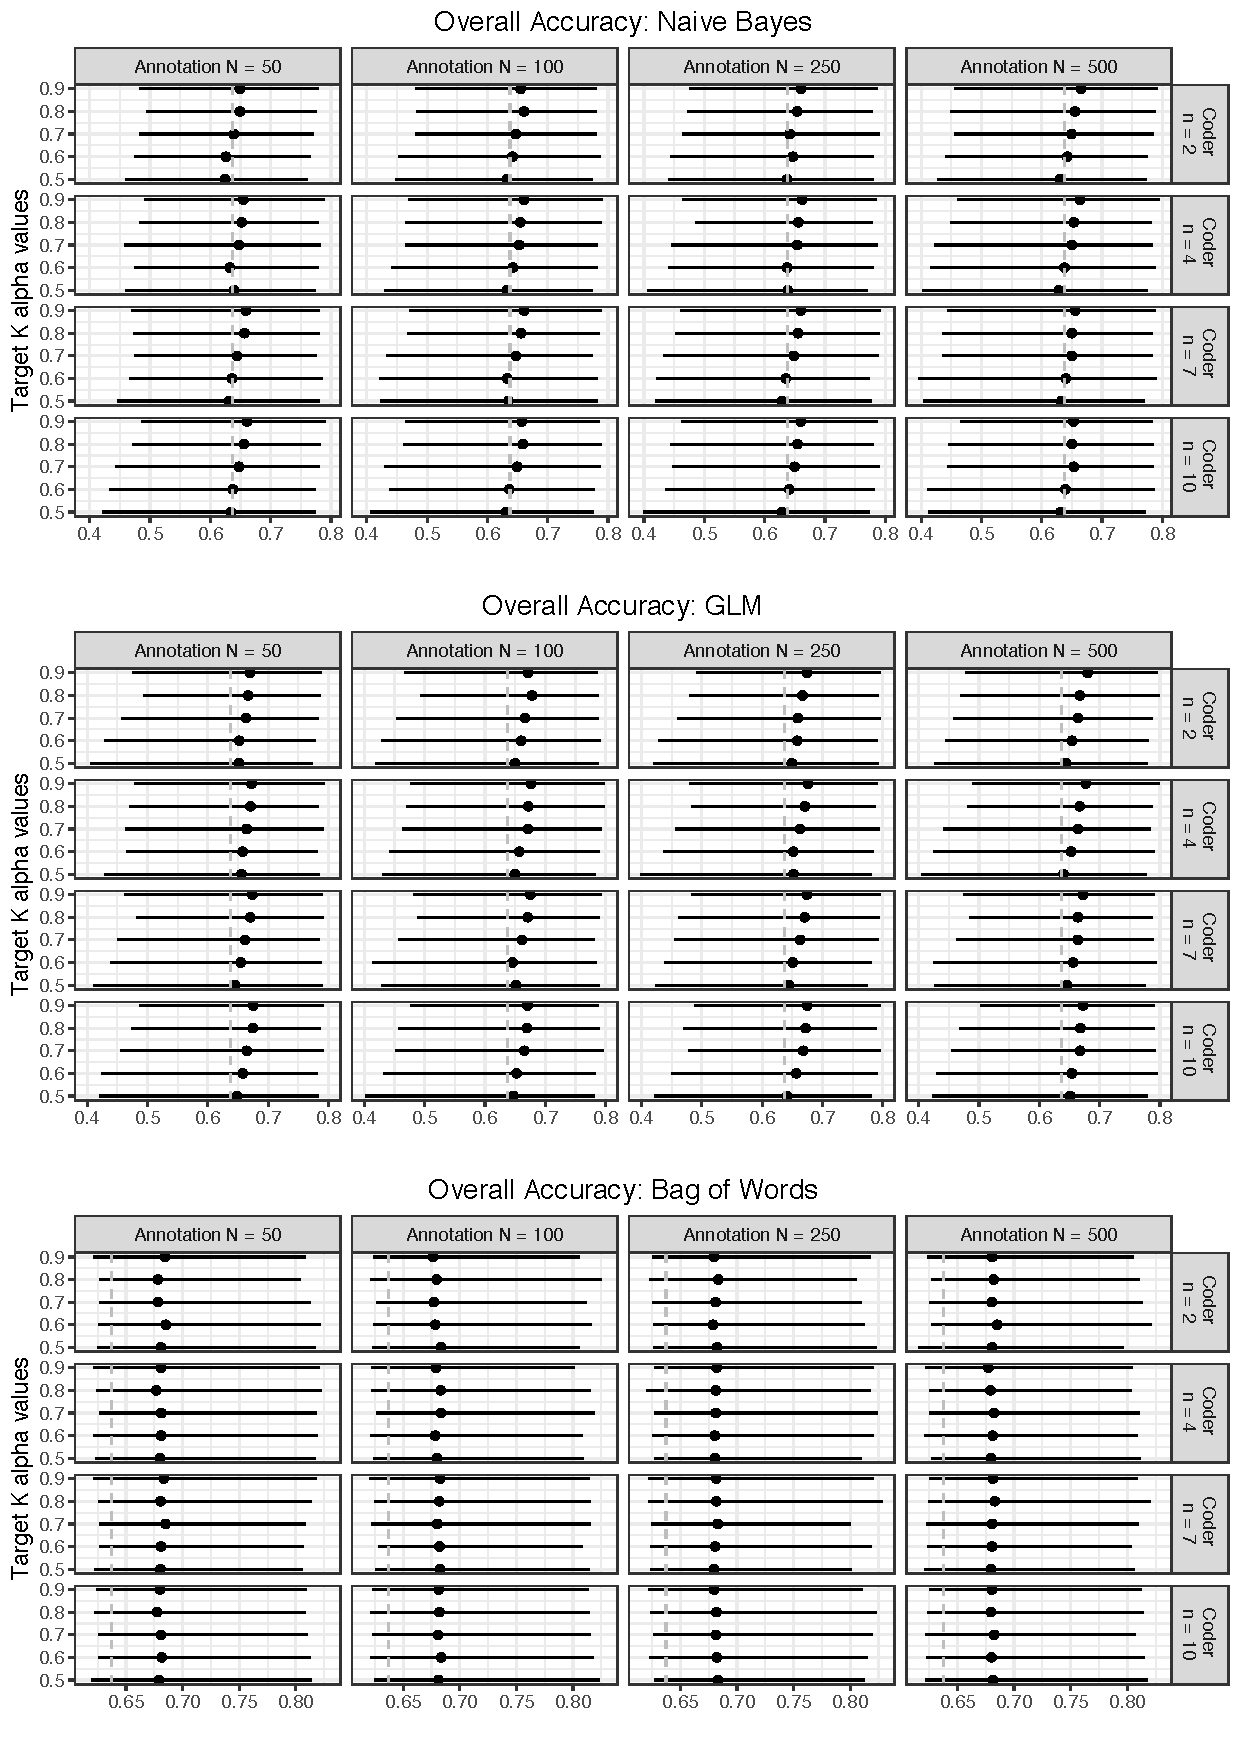
\includegraphics[trim={0.2cm 0.2cm 0.2cm 0.2cm}, clip, width=\columnwidth]{Results/overall_accuracy.pdf} 
         \captionsetup{format=hang}
         \caption{Overall classification accuracy against true value across conditions (Reference line is overall mean).} 
         \label{fig:Figure1}
\end{figure}    

As can be seen in Figure \ref{fig:Figure1} above, within two ML scenarios, using \enquote{better} quality training material appears to directly increase true classification accuracy, which is expected results. Using the overall accuracy in our simulation as the reference point, the first and the second panels of Figure \ref{fig:Figure1} makes it clear that the reliability level of training material has a nontrivial benefit in improving the accuracy of prediction based on automated procedures. Indeed, this is somewhat expected results since the ML methods takes the human input as the basis for developing the classification algorithm, therefore overall accuracy of the final classifier is dependent upon human input and its quality thereof. In contrast, the last panel of Figure \ref{fig:Figure1} shows that a typical Bag-of-words application does not benefit from improved (post-hoc) human coding. Yet again, this is a much expected pattern, since the quality of a given dictionary itself does not depend at all on \textit{post-hoc} validation of human coding unless manual coding is directly utilized in developing and constructing dictionary itself. Overall, our results presented in Figure \ref{fig:Figure1} show that our simulation setup can correctly reproduce a common pattern in extant studies (therefore ensures the validity of our analysis and conclusion).   

Next, we examine indirect consequences of relying on imperfect human coded materials as a benchmark in evaluating the performances of automated procedures in terms of post-hoc validation. Typically, researchers rely on a small fraction of human-coded materials for validating their primary findings from automated procedures, deciding whether the overall accuracy or classification performance is good enough to proceed to further analyses, based on some \textit{a priori} chosen threshold value: if validation (based on human coding) is purportedly not satisfying enough to pass such a threshold level, additional steps are sought to improve the quality of automated procedures (e.g., re-training of algorithms, or changing the dictionary, etc).\footnote{Here, we do not consider a scenario where a researcher decides to improve the quality of human coding. This is based on the consideration, as to our argument being advanced here, that a researcher (often incorrectly) assumes that human coding is perfectly reliable and valid.} The primary interest of such post-hoc validation procedures lies in extrapolating the observed level of classification performance (based on validation materials) to the level of classification performance \textit{that could have been observed} based on the entire range of data. In other words, the observed level of classification performance serves as a proxy, or an estimate for the true, unknown classification performance. Therefore, an interesting question here is how well the observed classification performance reflects true classification performance under imperfect reliability, and how large or small a potential bias is. Relatedly, making decisions about the unknown, true values of overall classification performance based on observed performance from hand-coded validation materials, essentially, can be seen as classical decision error scenarios (i.e., type I and type II errors), as schematically presented in Table \ref{tab:Table2}.
\centerline{ -- Table \ref{tab:Table2} about here -- }    

% Table 1 and 2.
\begin{table}[!htbp] \centering 
	\begin{minipage}{\textwidth}
    \centering
  \caption{\\ Results of the systematic literature review} 
  \label{tab:Table1} 
\begin{tabular}{@{\extracolsep{5pt}} cccccc} 
\\[-1.8ex]\hline 
\hline \\[-1.8ex] 
 \textbf{Method} & \textbf{Total} & \textbf{Refer to} &  \textbf{Report} & \textbf{Refer to} & \textbf{Report} \\ 
 \textbf{Used} & & \textbf{Gold Standard} & \textbf{Reliability} & \textbf{Validation} & \textbf{Val measures} \\
\hline \\[-1.8ex] 
 Dictionary & 55 & 29 (53\%) & 9 (16\%) & 27 (49\%) & 21 (38\%) \\
 Supervised ML & 18 & 16 (89\%) & 10 (56\%) & 15 (83\%) & 12 (67\%) \\
\hline \\[-1.8ex]  
\end{tabular} 
\begin{tablenotes}[para,flushleft]
\small \vspace{0.15in}
\textbf{Note:} Percentages refer to share of articles using that method.\\ 
\end{tablenotes}
 	\end{minipage}
\bigbreak
\vspace{0.5in}
 	\begin{minipage}{\textwidth}
    \centering
\caption{\\ Decision scenarios based on observed vs. true level of classification performance.} 
  \label{tab:Table2} 
  \begin{tabular}{ ccc}
\toprule
      \multicolumn{1}{c}{} & \multicolumn{2}{c}{\textbf{True classification performance}} \\
\cline{2-3}
   \textbf{Observed} & Below threshold & Above threshold \\
\hline \\[-1.8ex] 
 Below threshold & True Negative & False Negative (Type II) \\ 
 Above threshold & False Positive (Type I) & True Positive \\ 
\hline \\[-1.8ex]  
  \end{tabular}
  \end{minipage}
\end{table} 

In order to illuminate the potential consequences of relying on imperfect data in making decisions about the true, unknown classification performances of the proposed automated procedure, we divide our entire simulations into four mutually exclusive categories, as in Table \ref{tab:Table1}, based on the cross-tabulation of \enquote{observed} F1 scores (from validation materials) against true F1 scores (based on the true values of y). We first present the proportion of simulation cases which incorrectly conclude about the overall classification quality based on observed quality. Second, we further present the degree of relative \enquote{bias} within such incorrectly concluded cases --- defined as the $ F1_{validation}/F1_{true} $, where F1 score is a weighted average of the precision and recall --- which captures the degree of under- or over-estimation of (true) overall F1 scores against observed F1 scores based on human validation materials. For this application, we choose the cutoff value of F1 score to be 0.6478, which is just the average F1 score reported in Study 1.
\centerline{ -- Figure \ref{fig:Figure2} to Figure \ref{fig:Figure4} about here -- }    

% Figure 2 proportion of decision error, Naive Bayes
\begin{figure}
\captionsetup[figure]{labelfont={bf,it}}
    \centering
    \begin{subfigure}[t]{0.95\textwidth}
        \centering
        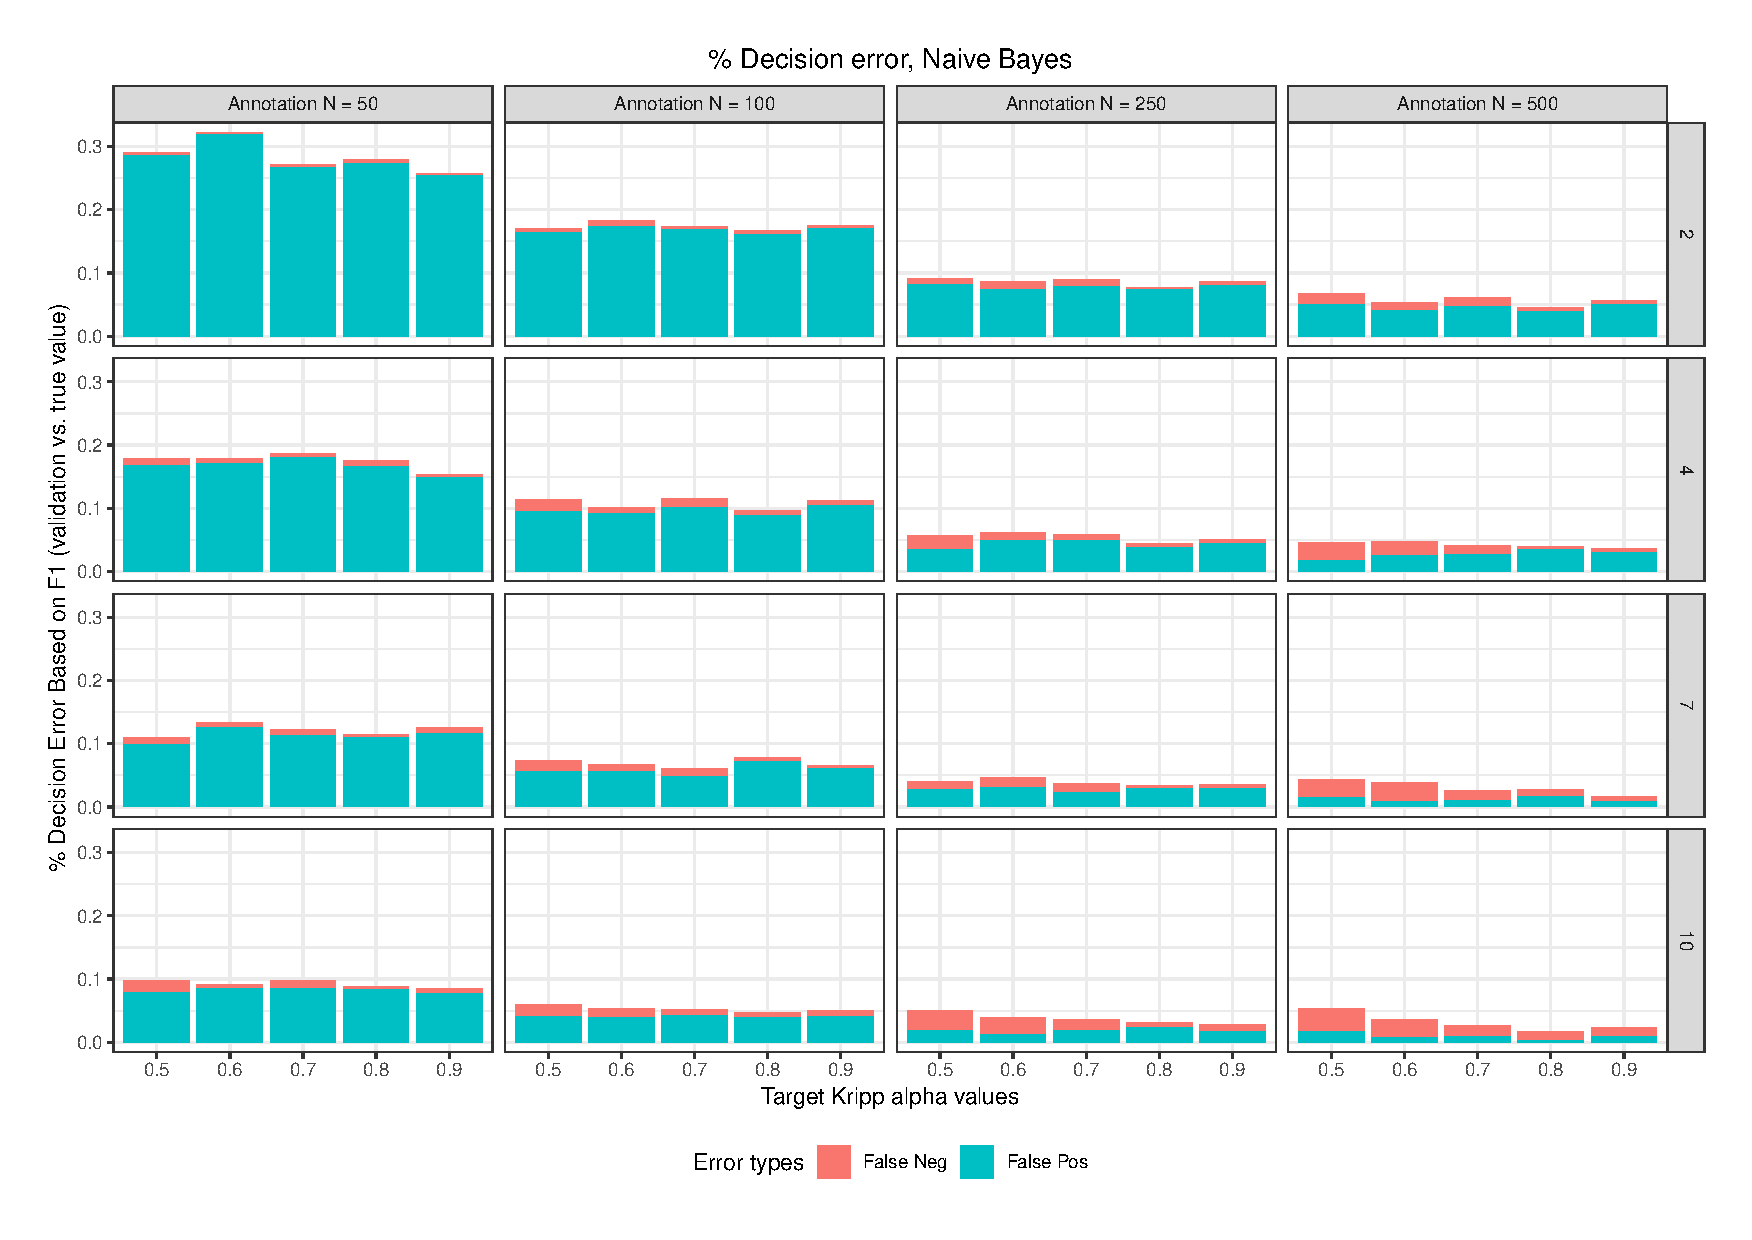
\includegraphics[clip, width=\linewidth, page = 1]{Results/BAYES_summary_05.pdf} 
    \end{subfigure}
    \begin{subfigure}[t]{0.95\textwidth}
        \centering
        \captionsetup{font=small}
        \includegraphics[clip, width=\linewidth, page = 2]{Results/BAYES_summary_05.pdf} 
    \end{subfigure}
    
    \captionsetup{format=hang}
    \caption{Percentage of decision error and relative bias in F1 scores (over 1000 Simulations per each scenario), Na\"{\i}ve Bayes classifier.} 
    \label{fig:Figure2}
    \captionsetup{font=small}
    \caption*{Note: Upper panel = Proportion of cases (each simulation run) incorrectly conclude on classification performances. Lower panel = Relative bias in F1 scores among 1000 replications, with their median and 95\% percentile confidence intervals.}
\end{figure}          

% Figure 3 proportion of decision error, GLM
\begin{figure}
\captionsetup[figure]{labelfont={bf,it}}
    \centering
    \begin{subfigure}[t]{0.95\textwidth}
        \centering
        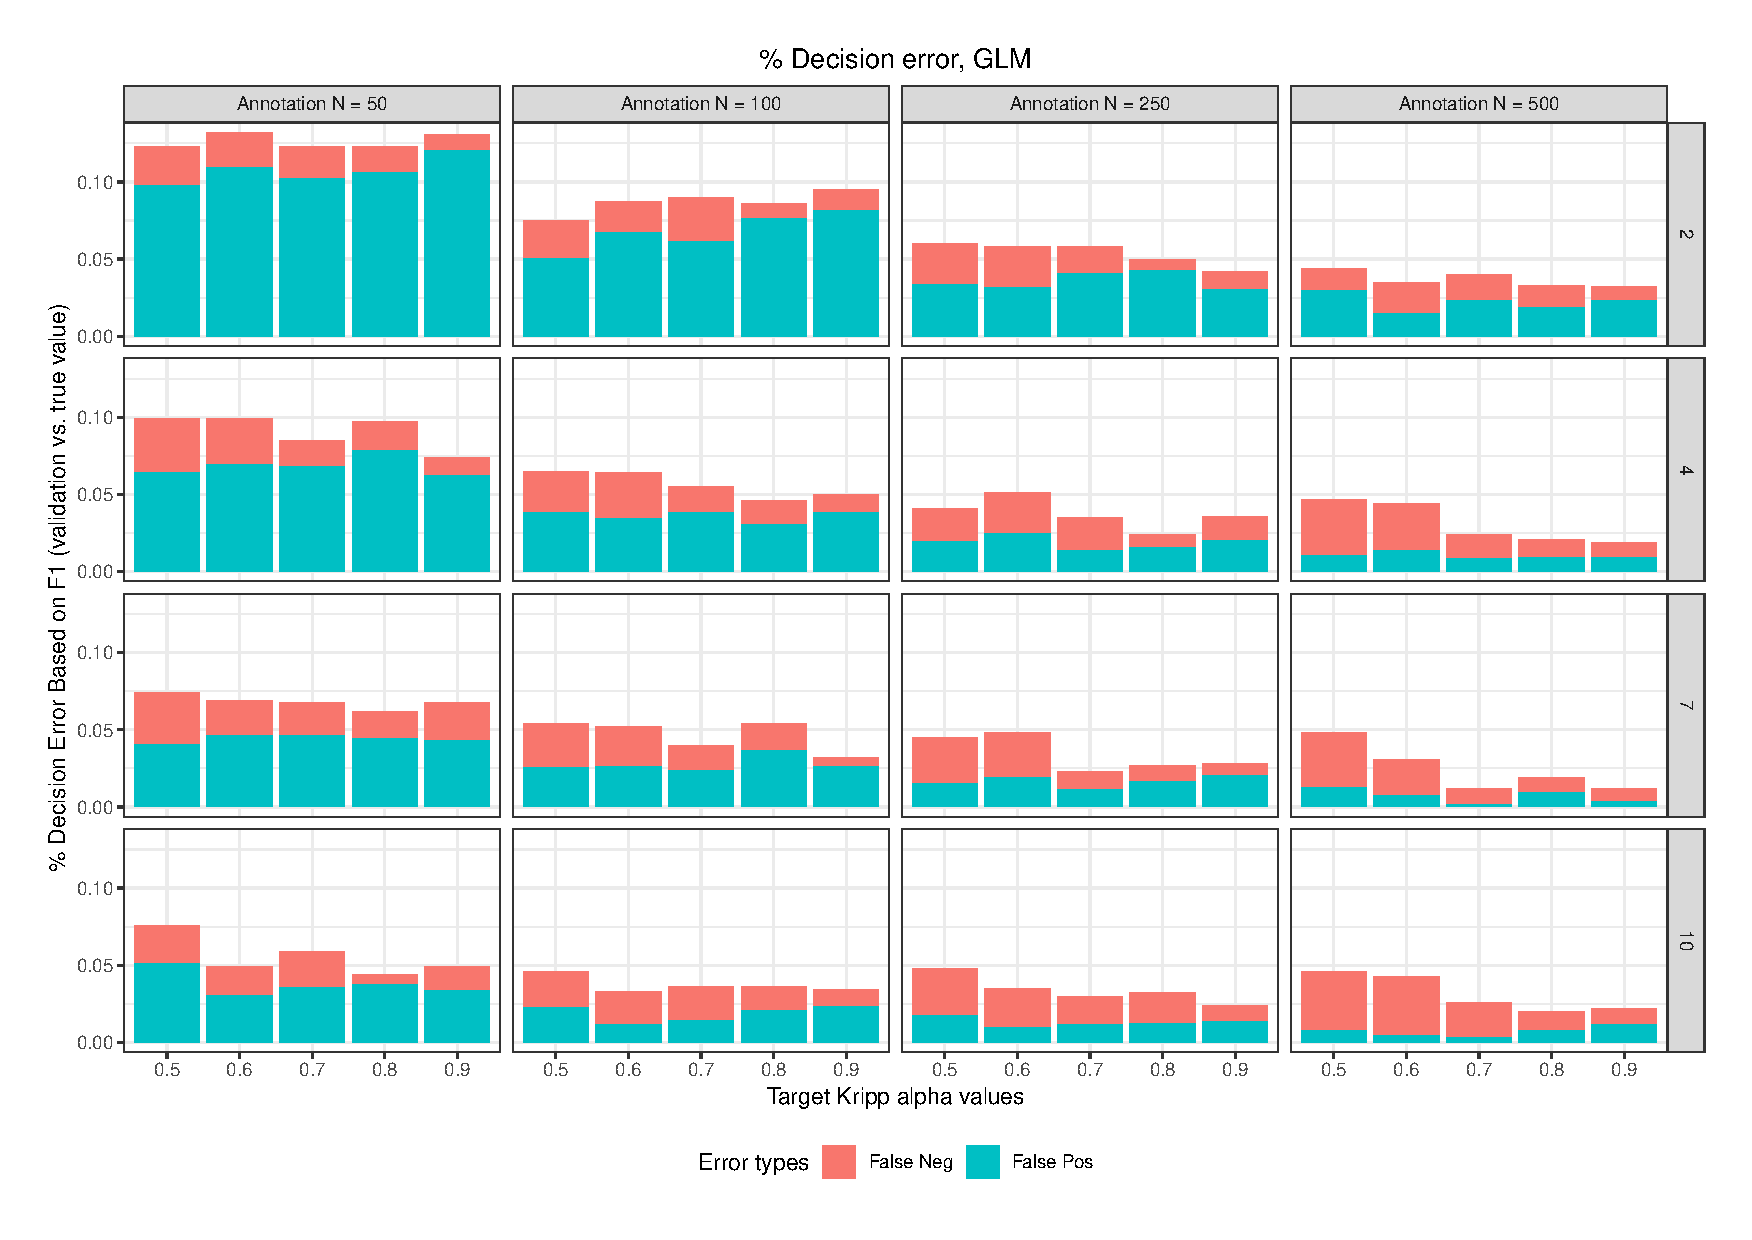
\includegraphics[clip, width=\linewidth, page = 1]{Results/GLM_summary_05.pdf} 
    \end{subfigure}
    \begin{subfigure}[t]{0.95\textwidth}
        \centering
        \includegraphics[clip, width=\linewidth, page = 2]{Results/GLM_summary_05.pdf} 
    \end{subfigure}
    
    \captionsetup{format=hang}
    \caption{Percentage of decision error and relative bias in F1 scores (over 1000 Simulations per each scenario), GLM classifier.} 
    \label{fig:Figure3}
    \captionsetup{font=small}
    \caption*{Note: Upper panel = Proportion of cases (each simulation run) incorrectly conclude on classification performances. Lower panel = Relative bias in F1 scores among 1000 replications, with their median and 95\% percentile confidence intervals.}
\end{figure}     

% Figure 4 proportion of decision error, BoW
\begin{figure}
\captionsetup[figure]{labelfont={bf,it}}
    \centering
    \begin{subfigure}[t]{0.95\textwidth}
        \centering
        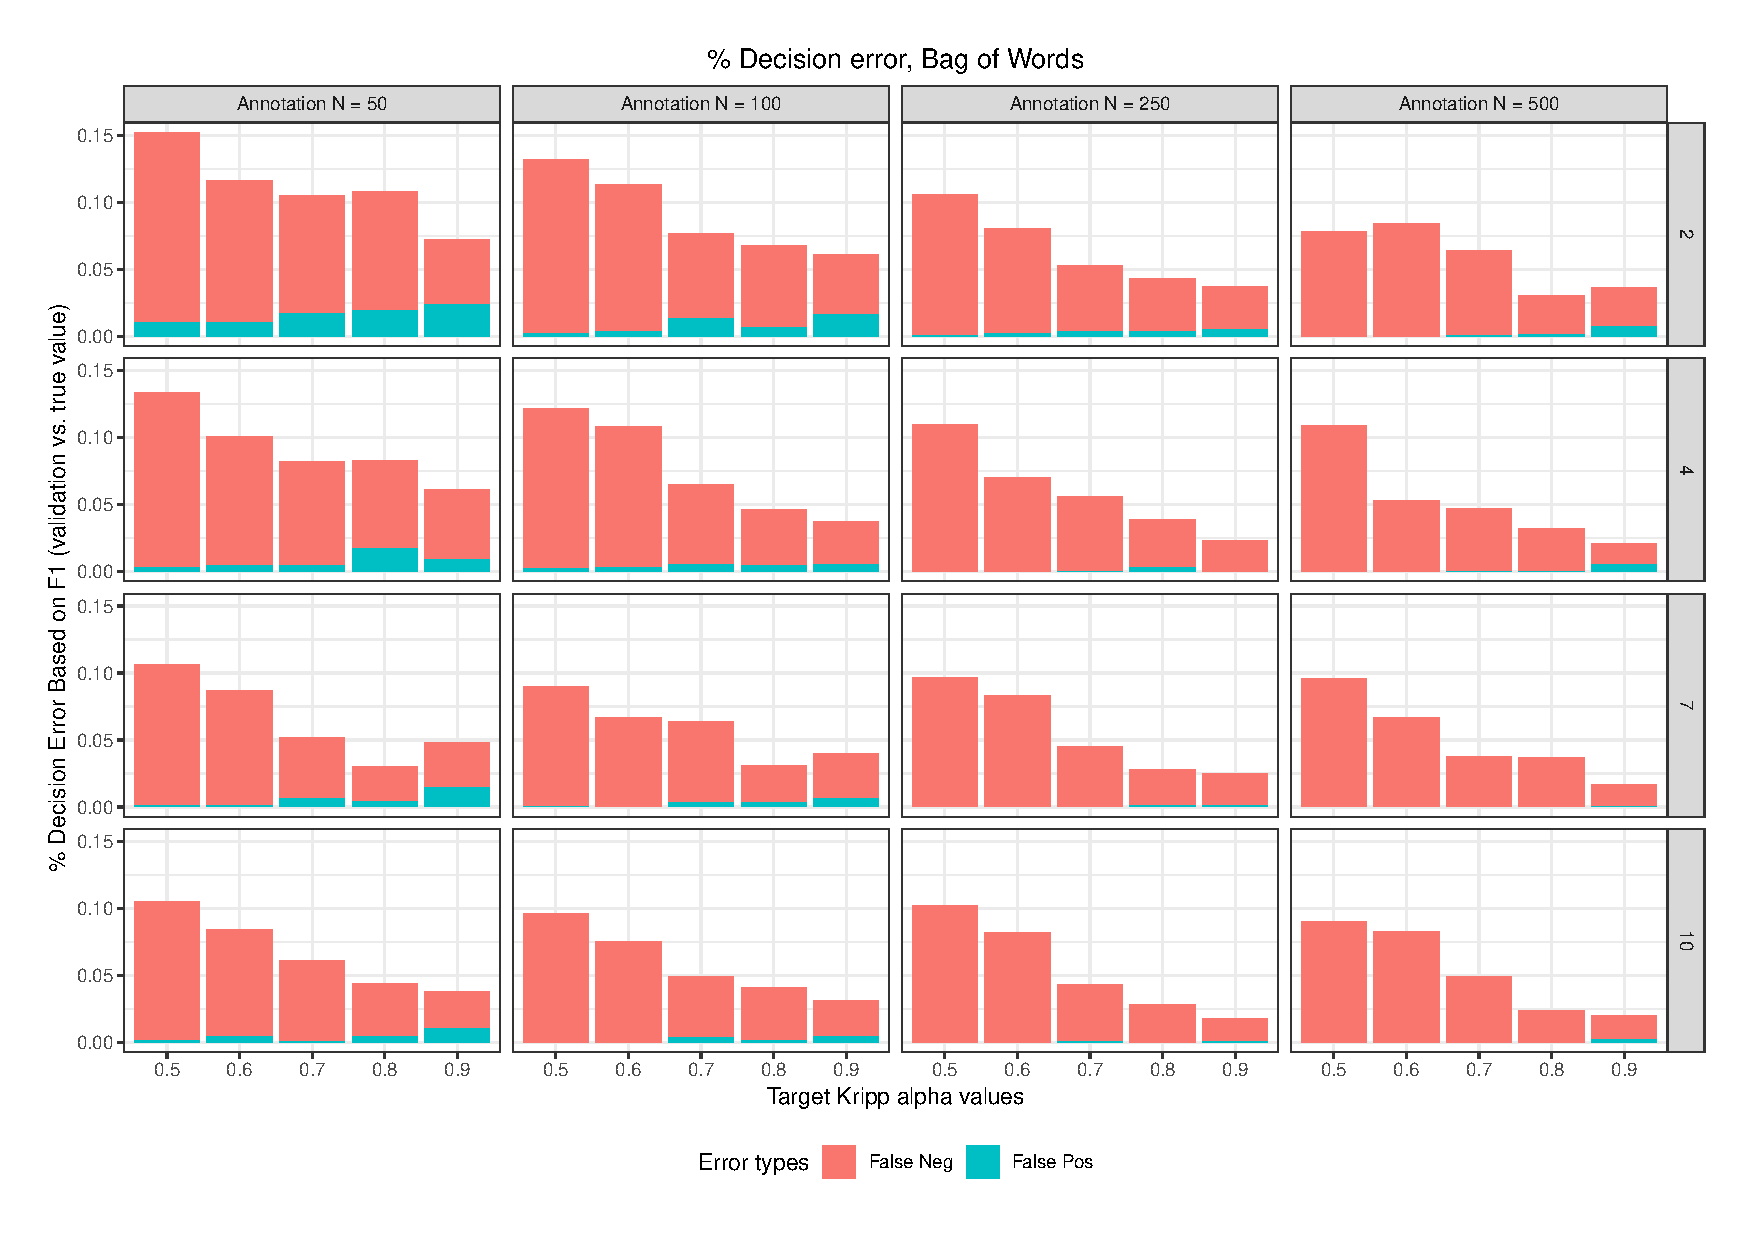
\includegraphics[clip, width=\linewidth, page = 1]{Results/BoW_summary_05.pdf} 
    \end{subfigure}
    \begin{subfigure}[t]{0.95\textwidth}
        \centering
        \includegraphics[clip, width=\linewidth, page = 2]{Results/BoW_summary_05.pdf} 
    \end{subfigure}
    
    \captionsetup{format=hang}
    \caption{Percentage of decision error and relative bias in F1 scores (over 1000 Simulations per each scenario), Bag-of-words.} 
    \label{fig:Figure4}
    \captionsetup{font=small}
    \caption*{Note: Upper panel = Proportion of cases (each simulation run) incorrectly conclude on classification performances. Lower panel = Relative bias in F1 scores among 1000 replications, with their median and 95\% percentile confidence intervals.}
\end{figure}     

    As can be seen through Figure \ref{fig:Figure2} to \ref{fig:Figure4}, it appears that utilizing more \enquote{high-quality} materials for post-hoc validation has obvious and discernible consequences in the evaluation of classification quality of the automated procedures. Among 1000 replications of each scenario, all of our experimental factors appear to decrease the decision error rates (i.e., using observed level of F1 scores to approximate the true F1 score). The leftmost upper panel in Figure \ref{fig:Figure2} shows that in worst-case scenarios in which using only two coders with a handful of materials, coupled with low reliability (K alpha of 0.5), such suboptimal hand-coded data result in approximately 30\% of cases incorrectly over- or underestimate the true F1 scores. Under the same combination of the total number of coders and independent annotations per each coder, improving reliability at best marginally decreases the overall percentage of decision errors. Yet as either a total number of coders or a number of independent annotations per each coder starts to increase, we see that the total proportion of cases that incorrectly estimate the true F1 scores start to decrease substantially (the upper panel of Figure \ref{fig:Figure2}) while the relative bias (the bottom panel of Figure \ref{fig:Figure2}) also starts to converge to true estimates, both in ML scenarios and dictionary approaches. While there appears no apparent overall main effect of higher reliability in terms of reducing the total number of decision error in ML approaches, using higher reliability manual validation materials tends to \textit{reduce} the magnitude of relative bias (i.e., the degree under- or overestimation of the true F1 scores based on observed F1 score), greatly reducing the uncertainties regarding the ultimate conclusions based on automated procedures. In bag-of-words applications as presented in Figure \ref{fig:Figure4}, we see more clear impact of higher reliability in reducing potential decision error using observed F1 scores. While it appears that using observed classification quality derived from manually coded validation materials in bag-of-words applications tend to underestimate the true classification quality (lower panel of Figure \ref{fig:Figure4}), higher reliability in such validation material nevertheless reduces the uncertainties regarding the ultimate conclusions based on automated procedures. This provides much consistent pictures of the impact of \enquote{quality} of manually coded materials in validating the conclusions derived from automated procedures.   

\section{Discussion and Conclusion}
    
    The aims of the current investigation were twofold; first, we attempted to provide a systematic overview of current practices in validation procedures of automated content analysis in the social sciences. Second, we aimed to provide further insights into how the various decisions taken by researchers on various steps of the research process (specifically, test and training set preparation, and algorithm validation phases) influence the overall conclusion and quality of arguments that could be drawn from the analyses of such data. In order to achieve these goals, Study 1 relied on a systematic review of published papers from major social science journals that purportedly have relied on \enquote{automated text analysis.} The results of the first study show that, while automated content analysis procedures are widely used throughout social science applications, there is still strikingly little consistency in \textit{whether} and \textit{how} validation is reported. Very often, studies do not report \textit{any} validation metrics when relying on automated methods. Even when they do, metrics related to (human-coding based) validations are generally not consistently reported, and are often limited in providing actual methodological details. For the second study, we have designed a set of Monte Carlo simulation procedures, which closely mimic multiple scenarios of data coding, classification, and data validation for the most widely-used supervised learning-based applications as well as for the dictionary classification methods. The second study revealed that any decision taken during preparation of validation materials -- a number of coders, a size of the training sets produced by each coder, and the \enquote{quality cut-off point} (e.g., Krippendorff's alpha for intercoder reliability) -- indeed all produces systematic consequences for the evaluation of the proposed automated procedures. 

    Coupled together, the results from both studies give good reason for concern for the quality (or rather the \textit{validity}) of conclusions drawn from automated content analyses in the social sciences. In order to make sensible conclusions from data, a proper validation of the proposed automated methods is much needed. A statistical model may have an excellent fit to the data and a chosen dictionary may very well recover some pre-defined categorizations, but these metrics themselves do not provide any sensible meanings for their own if the model suffers from over-fitting the training data, or the pre-defined dictionary does not actually conceptually \enquote{align} with the categories of interest. To be clear, the current study \textit{does not} make a case for the argument that we should \textit{exclusively} rely on human validations. Quite contrary, one of the main points being advanced here is that humans are not perfect --- however, this study argues that validation is essential in general. Researchers should still validate their methods either against some pre-existing, \enquote{established} categorization, or against the (potentially imperfect) human \enquote{gold-standard}; while the \enquote{gold-standard} is the best we can get, the results of this study suggest that extra cautions should be taken when manual human annotations are involved in such validation procedures. Often, imperfect judgment of human coding can percolate to machine coding to inferences if a researcher turns a blind eye to such imperfect quality of human judgment. We therefore advise researchers to pay close attention to the issue of proper reliability in manually coded validation materials in order to reduce uncertainties in potential biases, while strives to increase the overall size of the validation materials as large as possible in order to reduce overall decision errors based on manual validation materials.    

    Few limitations should be noted. First, we only have considered a binary classification in our simulation setup while only focused on a single dimension of validation metrics --- specifically, recall, precision, and resulting F1 scores. While this greatly simplifies our main arguments and (still complex) simulation setups, there are indeed a nontrivial number of existing applications that go beyond such simple classifications, dealing with numerical forms of predictions (i.e., scaling). Ultimately our conclusion would be of course bounded to our specific setup, yet we reason that our core arguments can be equally applicable to more complex forms of automated content analysis applications (and potentially to any unsupervised methods). Given the additional complexity of such judgments, we suspect the potential negative impacts of imperfect quality of validation materials should be greater, if not identical, on those applications. 

    Designing a simulation-based study gives us a unique opportunity to see the many potential, \textit{what if} scenarios of the research processes. Such an approach, if carefully designed, allows to robustly explore potentially important variability in research processes in a probabilistic manner without having to actual spend resources on carrying out those multiple scenarios. Also, one of the core advantages of relying on simulation approach is that a researcher has the ability of \enquote{knowing the truth,} specifically the true value of quantity of interest, $y$, as well as their correct functional forms that produce each observation (of media data) in this case. This also provides a mean for formally checking the sensitivity of one's findings, or able to provide a proper context of one's findings by exploring counterfactual scenarios. Such clairvoyance, however, comes at a cost --- the degree of abstraction and simplification. This simplification is done not only for computational, but also for conceptual reasons, however. As \textcite{scharkow2017measurement} note, \enquote{the challenge is to specify a simulation that is simple enough to be comprehensible, yet realistically models the underlying process of interest} (p. 330). In this regard, we have relied on somewhat idiosyncratic and simplified approaches in our simulations. While we surely acknowledge that our setup could have been constructed in a more realistic and complex way, our ability to accurately simulate human behaviour does not necessarily depends on very complex models. 

    Notwithstanding these limitations, we believe that our contribution would further prompt researchers both in communication science and the social sciences more generally to pay more closer attention to the issues of systematic validation of automated content analytic methods. Our contribution should be read as a call for a thorough and systematic application of validation procedures -- especially the one involves manually annotated materials as a \enquote{gold-standard}. Statistical models and algorithms, while being infallible in terms of reliability, are not inherently correct; they are only useful in so far as they can properly approximate researchers' conceptualizations. And this degree of approximation, we argue, can only be established after thorough and systematic validations. In this regard, it is worth stressing here that automated content analysis also takes (and should take) time and resources, not just regarded as a cheap alternative to expensive manual coding. Taking into account the time and/or resources needed to design proper studies and inferences thereof, a little extra time spent on proper validation would pay off, ensuring that the conclusion drawn from such studies do not start to stink.

    
\printbibliography
%\newpage
%\begingroup
%\parindent 0pt
%\parskip 1ex
%\def\enotesize{\normalsize}
%\theendnotes
%\endgroup
\end{document}
